Evaluation of the vocabulary list generation approaches is challenging:
The accuracy of the approaches is evaluated by evaluating the efficiency of the vocabulary lists.
We have described in detail our approach to vocabulary efficiency evaluation in Section \ref{sec:experimental-setup-with-ai}, which involves running an AI model on a context-specific corpus with a given vocabulary, where the vocabulary is given by taking the first n $k$ words from the vocabulary list in question.
However, this approach is very similar to our approach for list generation, which involves analyzing AI interaction of AI models with corpora through the use of XAI methods.
Therefore, it is natural to assume that our evaluation approach is biased towards the lists stemming from our list generation approach.
This concern is especially pertinent as it has been shown that AI models do not reliably respond comparably to humans when the inputs to NLP tasks are perturbed \cite{tjuatjaLLMsExhibitHumanlike2024}.

To the best of our knowledge, there has not yet been a proposed evaluation metric for vocabulary lists that can be done automatically and which outputs a simple numeric result.
For this reason, in addition to our own evaluation approach utilizing AI models, we take some sample vocabulary lists, use our evaluation approach, and check whether the results align with human intuition.

For this reason, our evaluation is not only concerned with analyzing statistics of measured efficiency, but also with whether the calculated efficiency values are reliable.
The questions examined in this chapter can be summed up as:
\begin{enumerate}
	\item Does the efficiency evaluation of our list correspond with human intuition?
	\item Does our generation approach outperform frequency-based approaches?
	\item What are the upsides/downsides of each list generation approach (accuracy, speed, free choice of corpora)?
	\item How can the various approaches be combined to supplement each other's weaknesses?
\end{enumerate}

\todo{Add section references when chapter structure is fixed}
The following sections first describe the (numeric) metrics used in the evaluation.
We then introduce several baselines against which we compare our list generation approach.
The baselines include both publicly available vocabulary lists from online language learning tools, and existing list compilation methods introduced in Section \ref{sec:frequency-based-list-generation-methods} in connection with the corpora used for our own lists for a more direct comparison.

We then present the results of the evaluation, as well as discuss their implications.

\section{Evaluation Measures}

The various utility extraction approaches produce ranked lists as outputs.
To compare these, we employ both quantitative and qualitative comparison approaches, described in the following sections.

\subsection{NLP Task Performance}
Our primary metric for evaluating a vocabulary list's efficiency is the approach explained in Section \ref{sec:list-generation}:
We let an AI model perform an NLP task with a vocabulary consisting of the first $k$ elements of the list.
The limited vocabulary is simulated by removing words outside the vocabulary from the inputs to the model.
We then progressively increase the vocabulary by increasing index $k$ until we reach the end of the list.
The increase of vocabulary size is exponential, as this ensures a quick evaluation and performance is expected to not grow very much towards the end of the list, where the less useful words should be (this assumption can be confirmed in the evaluation results in Section \ref{sec:results}).

Listing \ref{alg:efficiency-evaluation} shows pseudocode for the described setup:

\todo{Edit surrounding descriptions of efficiency to be in line with pseudocode}

\todo{
	Explain that a performance score between 0 (worst input) and 1 (unaltered input) is used for normalization.
}
\begin{algorithm}
\caption{Efficient List Generation}
\label{alg:efficiency-evaluation}
\begin{algorithmic}[1]
\Require voc\_list, corpus, model
\State Initialize $vocabulary \gets \emptyset$
\State Initialize $scores \gets []$
\State Set $test\_interval \gets 100$

\For{$i \gets 0$ to $\text{length}(voc\_list)$ step $test\_interval$}
    \State Add $voc\_list[i]$ to $vocabulary$
    \State Initialize $line\_scores \gets []$
    
    \For{each $line$ in $corpus$}
        \State $line\_with\_only\_known\_words \gets$ mask\_words\_not\_in\_vocabulary($line$, $vocabulary$)
        \State $baseline \gets$ model($line$)
        \State $model\_output \gets$ model($line\_with\_only\_known\_words$)
        \State $score \gets$ similarity($baseline$, $model\_output$)
        \State Append $score$ to $line\_scores$
    \EndFor

    \State $avg\_score \gets$ average($line\_scores$)
    \State Append $avg\_score$ to $scores$
\EndFor

\end{algorithmic}
\end{algorithm}


This approach gives us a direct, quantitative metric for the efficiency of a vocabulary list.

As an illustration, we present the results of one such efficiency evaluation run on a corpus can be seen in Figure \ref{fig:marlon-brando-eval}.
\begin{figure}[H]
	\centering
	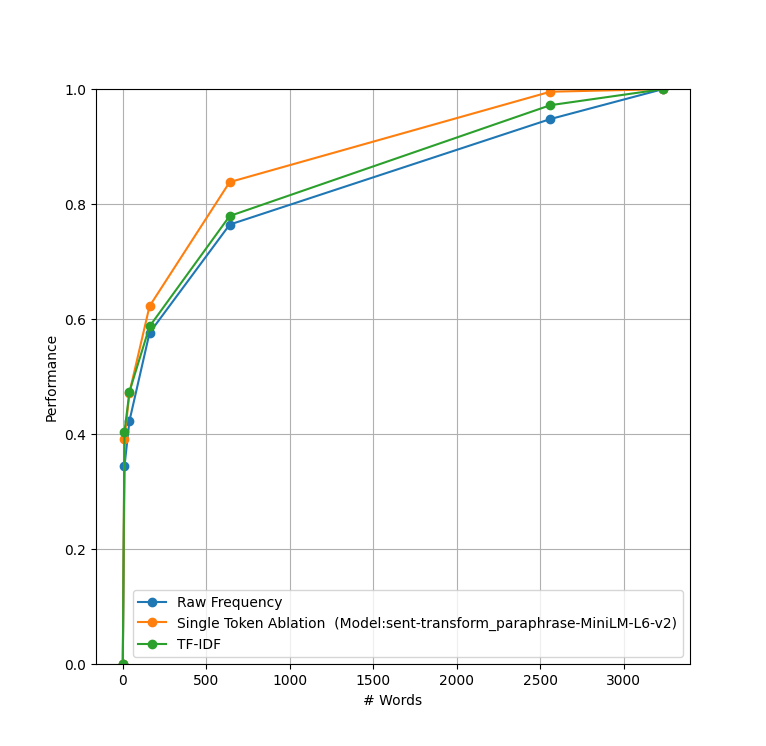
\includegraphics[width=0.5\textwidth]{marlon-brando-eval.png}
	\caption{Efficiency evaluation results on vocabulary lists for the Wikipedia Article of American actor Marlon Brando \protect\footnotemark.}
	\label{fig:marlon-brando-eval}
\end{figure}

\footnotetext{\url{https://en.wikipedia.org/wiki/Marlon_Brando}}

To make the figure readable, only three list generation approaches are compared, namely Raw Frequency, TF-IDF, and Single Token Ablation with the sentence embedding model.
The vocabularies are evaluated with an initial size of 10, and increase by a factor of 4 in each step, until a final evaluation is done with the full vocabulary list.
The full list typically contains all words from the corpus, which is why the performance reaches 1 with all lists.

To compare the results on a broader scale, we aggregate the results of the evaluation runs for each corpus type, word utility evaluation method and AI model (where applicable) by taking the average performance of the generated vocabulary list, with vocabulary sizes 0, 10, 40, 160, and 640.


\todo{Describe train/test splitting}
When we find two approaches for list generation produces vocabulary lists of similar efficiencies, we might ask ourselves if these lists are similar:
Can two lists which differ substantially in their ordering produce similar performance?
To answer this question, the next section introduces additional evaluation metrics which measure the similarity of two lists.

\subsection{List Similarities}
In order to compare the resulting vocabulary lists provided by the various approaches, metrics are needed that can be consistently calculated across the different approaches.
While a human may be able to qualitatively analyze lists and gain a rough idea of their similarity, computed metrics provide an instantaneous (if simplified) outlook on similarities.
A metric shall be defined as a function which takes as parameters two word lists of equal length which are word lists ordered in descending order by supposed utility, and outputs a real number giving either a distance or similarity between the lists.

Considerations of the choice of metric are:

\begin{description}
	\item [Handling of lists with partial overlap.]
	      Metrics must be able to handle elements which occur in only one of the two lists.
	      Thus, a metric which solely compares ranks of elements is not viable.
	\item [Start of lists is more impactful than end.]
	      Since the beginning of lists contains the words which are ranked as most important, changes at the top should impact the metric more than changes at the bottom. This includes (1) Equal differences in rank should be counted as more important if they occur further up the list.
	      A word that is rank 1 in list A, but rank 101 in list B says more about the similarity than if a word is rank 2000 in list A, but rank 2100 in list B. Likewise, if a word is absent from list B, it implies a greater difference if that word is at rank 1 in list A than if it were at rank 1000.
\end{description}

\subsubsection{Metrics Used}

\begin{description}
	\item [Sequential rank agreement (modified)] \cite{ekstromSequentialRankAgreement2015}: This metric is based on the deviations of some subset of the lists in the upper ranks.
	      It is important to note that this metric has an additional parameter "depth" which determines how many elements (from the top of the list) are considered.
	      It is therefore more helpful to view its results at various depths.
	      The original formula for this metric in the case of two lists is:
	      \[
		      a_{d} := a \text{ from start to rank } d
	      \]

	      \[
		      S_{d} := a_{d} \cup b_{d}
	      \]

	      \[
		      SRA_{d}(a, b) := \lambda \cdot \frac{\sum_{x \in S_{d}} \sigma ^2 \left( \left( r_{b}(x) \right) - \left( r_{a}(x) \right) \right)}{|S_{d}|}
	      \]

	      where \(\lambda\) is a normalization factor ensuring that \(\max(SRA) = 1\).
	      In its proposed form, this metric can only compare lists which contain the same set of unique elements, just in different orders.
	      In order to make it work on lists where this is not the case, one can set the "rank" of nonexisting elements to a value greater than the length of the lists, such as \(2 |a|\).
	      Another drawback of the metric is that the standard deviation of two numbers does not depend on their absolute value, only their difference.
	      However, to satisfy number 3 of the stated requirements, we can take the deviation of the logarithm of the ranks instead of the deviation of the ranks themselves, resulting in the formula

	      \[
		      r^{\prime}(x) :=
		      \begin{cases}
			      \mathrm{rank}_{b}(x) & \text{if } x \in b, \\
			      2 \cdot |a|          & \text{otherwise.}
		      \end{cases}
	      \]

	      \[
		      SRA^{mod}_{d}(a, b) := \lambda \cdot \frac{\sum_{x \in S_{d}} \sigma ^2 \left( \log (r^{\prime}_{b}(x))-\log(r^{\prime}_{a}(x))\right)}{|S_{d}|}
	      \]

	      For this modified version, \(\lambda\) can be calculated with:

	      \[
		      \lambda = \frac{1}{SRA_{d}(a, a^{*})},
	      \]

	      where \(a^{*}\) is a list such that \(a \cap a^{*} = \emptyset\).
	      % \item \textbf{Average overlap / rank-biased overlap} \cite{webberSimilarityMeasureIndefinite2010}: Compares ranked list and puts more emphasis on the top of the list than at the bottom. However, assumes that the elements of both lists are the same, i.e., that all elements of list A are also in list B and vice versa.
	      %
	      % \item \textbf{11-point interpolated average precision} \cite{manningIntroductionInformationRetrieval2008}: Uses set metric precision (though may also use recall or F1 score on various subsets of the list (first 10\%, first 20\% etc.) and takes their geometric mean to arrive at a single number.
	      %       As each of the elevent numbers is calculated on the partial subset of the list's elements starting at the first element, this means that changes in the top of the list affect more of these numbers and thus have a larger impact on the final calculated mean.
	      %       One drawback of this method is that precision measurement within the 10\% interval only takes into account set membership, not the order of words:
	      %       For a list containing 10,000 words, the evaluated intervals are words in the index intervals $\left[ 0, 1000 \right), \left[ 0, 2000 \right), ... ,\left[ 0, 10000 \right)$.  Differences of order within the first 1000 words are thus ignored.

	\item [Discounted Cumulative Gain]:
	      This formula outputs a value between 0 and 1, with 1 being given if both lists are identical, 0 when they have no elements in common, and values in between when there is partial overlap between elements and/or their order is different.
	      ${DCG_{p}} =\sum _{i=1}^{p}{\frac {rel_{i}}{\log _{2}(i+1)}}=rel_{1}+\sum _{i=2}^{p}{\frac {rel_{i}}{\log _{2}(i+1)}}$
\end{description}

\[
	rel_{i} :=
	\begin{cases}
		\frac{1}{rank_{b}(el_{i}) + 1} & \text{if } el_{i} \in b \\
		0                              & \text{otherwise}
	\end{cases}
\]
\subsubsection{Metrics Rejected}
\begin{description}
	\item [Kendall rank correlation ] \cite{kendallNEWMEASURERANK1938b}: This metric is bounded between 0 and 1 and compares the ranks of the elements of two lists. However, it cannot handle elements that only occur in one of the two lists, and thus is not suitable for our purposes. It also does not distinguish between differences in the upper and lower parts of the lists.
	\item [Spearman's footrule] \cite{spearmanCorrelationCalculatedFaulty1910}: Rejected for the same reasons as Kendall rank correlation.
\end{description}


\subsubsection{Tests of Applicability}
[Results of preliminary tests of various metrics on own lists such as rank switching ,replacement at bottom and top of list etc.]

\subsection{Sample text}
\todo{Show a sample paragraph with first n words from each list. Can be used to intuitively evaluate utilities}
In addition to the above automatic measures of list efficiency, we can also use human intuition to evaluate the various vocabulary lists:
To compare vocabulary list up to some index $k$, we use a sample paragraph, and take the vocabulary $V_{l, k}$ of each of the lists.
Then, we compare how the paragraph appears for each vocabulary if we blot out all words not in the vocabulary, in order to simulate the perspective of someone who only knows the words from the vocabulary.







\section{Baselines}
It may be useful to compare the lists generated by the various approaches with existing word lists from educational materials:
Textbooks often feature chapters with word lists, or sentences which can be converted to word lists with a tokenizer.
The purpose is to have a point of comparison, to see if generated lists agree with existing lists, and find reasons for differences.

\subsection{Existing Lists}
As one point of comparison, we can use existing vocabulary lists that are readily available in digital format, regardless of the method which created them.
For this, a survey was done on popular language learning tools which make public some of their learning data.



\todo{	Language learning textbooks}

\subsubsection{Duolingo}
While Duolingo is the most popular language learning application as of 2024, it does not publish its word lists or course contents that is free of cost and easily convertible to a format that can be processed with NLP tools.

\subsubsection{Rosetta Stone}
\Rosetta \footnote{\url{https://rosettastone.co.jp/}} is a popular online and mobile language learning platform.
\Rosetta\ publishes some of their course contents on its website \footnote{\url{https://support.rosettastone.com/s/article/Rosetta-Stone-Course-Content}}.
These lessons take the form of phrases that should help a learner to quickly gain competence in their target language.
To make a list of vocabulary from \Rosetta 's Lesson Contents, we use a tokenizer on the lesson and let the order of first appearance of a word in the lesson be its rank in the resulting vocabulary list.
Thus, the generated list features those words first which \Rosetta\ introduces first to its learners, which presumable is close to the word order that \Rosetta estimates is most useful.
One qualification of the previous statement is that some words are probably only introduced in order for the learner to have something concrete to talk about, rather than because of the word's inherent utility.



This section has introduced some pre-existing lists as points of comparison for our generated vocabulary lists.
However, one shortcoming of this comparison is that these lists have not been prepared with the same linguistic contexts in mind as those made by this work's approach, and thus their utility is naturally greater in general-context corpora than specialized ones.
While the context specificity of this work's utility extraction method is a major advance for creating vocabulary lists, it also makes this an unfair comparison.

However, apart from pre-existing lists, there also exist pre-existing \textbf{methods} of finding important words in texts, which we can also use as baselines to compare with our method.
These also use corpora, but not AI models or XAI methods to find important words.
The next section introduces some of these methods, which we use to generate comparison lists to our own.


\subsection{Existing List Generation Methods}
To get an impression of how well our XAI-based method for vocabulary list generation performs, it is informative to test established methods for extracting important words from texts.

\subsubsection{Raw Frequency}

Raw word frequency has been used as a criterion for which words to teach to language learners \cite{heChoosingWordsTeach2019}.
Frequency is much less computationally intensive than any of the XAI-based approaches, as it only requires a tokenizer to be run on a corpus, without involving model calls.

\subsubsection{Frequency, Without Stopwords}
One drawback of using raw frequency as the criterion by which to order vocabulary lists is that the most frequent words in most corpora consist of stopwords.
This can be seen in the following frequency word list from corpus [x].
\todo{insert sample from raw frequency word list from corpora used in experiments }

These words, while being the most generally useful, have very little meaning by themselves \cite{rajaraman2011data}.
For this reason, they are often filtered out in the inputs of NLP tasks.
Removing from the raw frequency-based word lists could be a way boost the list's  efficiency, especially at the top of the list.
We therefore filter out known stop words, based on a list from the popular NLP library \textit{NLTK} \footnote{\url{https://www.nltk.org/}}.
\footnote{The NLTK stopword list can be downloaded by following the instructions on \url{https://www.nltk.org/howto/corpus.html\#word-lists-and-lexicons}.}


\subsubsection{TF-IDF}
\todo{Either finish this section or replace with collection frequency normalization}
To characterize the contents of a document, \cite{qaiserTextMiningUse2018}.
TF-IDF has, to the best of our knowledge, not been considered for vocabulary list generation.
However, it is often employed to find key terms in a document, which characterize the document's contents with a small number of words.

TF-IDF: The frequency of a word in the context-specific corpus, normalized against a background corpus.

\subsection{LLM Prompts}
In recent years, Large Language Models have become a popular tools for language learners to find new words to learn about specific areas.
For this purpose, we run the following prompt to ChatGPT 3 for each context to get a sense of how well my method performs against this easy method.

Prompt:

\begin{lstlisting}[caption={Prompt given to the language model.}, label={lst:blade_runner_prompt}, captionpos=b]
	Given a learner of English who knows no English words so far:
Give me a list of 50 words from the script of the movie "Blade Runner" that they can learn, such that when reading the full script, they have the best understanding of what they are reading.
Order the list such that the most useful words appear at the top.
Do not group the words, just generate a raw list.
Do not number the bullet points. Do not put hyperlinks in the list.

\end{lstlisting}
\todo{results}

\section{Results} \label{sec:results}

\subsection{Correspondence of Efficiency Evaluation with Human Intuition}
As mentioned in the introduction to this chapter, we use the performance of AI models on corpora where we simulate a limited vocabulary in order to measure the efficiency of a vocabulary list.
Before we present the results of these tests, however, we must first establish that the performance of AI models is a reliable indicator that the list is useful to humans as well.
This section therefore examines several vocabulary lists tested on a corpus that should be familiar to most readers.

We compare the performances of the following lists:
\begin{enumerate}
	\item A list randomly selected from words in the corpus.
	\item A list compiled from raw frequency.
	\item A list compiled by single-token ablation.
\end{enumerate}

The full lists can be seen in the following table.
\todo{Insert table}

\subsection{Performance Results of Lists Generated from Same Corpus} \label{sec:results-same-corpus}

This section shows the results of our evaluation approach for the efficiencies of vocabulary list, applied to lists which have been generated by the various list generation approaches.
Performance scores were rounded to two decimals to improve readability.


Table \ref{tbl:performance-results} shows the aggregated results of small-scale corpora, separated by corpus type.
For small corpora, there is no train-test-data distinction, thus for each corpus and extraction method, a vocabulary list produced, whose efficiency is then evaluated with the same corpus as a basis.

\begin{table}[ht]
	\centering
	\begin{tabular}{llrrrrrrrr}
\toprule
 &  & \multicolumn{4}{r}{Performance} & \multicolumn{4}{r}{Performance ($\sigma$)} \\
 & Vocabulary Size & 10 & 40 & 160 & 640 & 10 & 40 & 160 & 640 \\
Generation Method & Generation Model &  &  &  &  &  &  &  &  \\
\midrule
Raw Frequency & - & 0.14 & 0.30 & 0.60 & 0.88 & 0.14 & 0.25 & 0.31 & 0.21 \\
\cline{1-10}
Average Reduced Frequency & - & 0.14 & 0.29 & 0.58 & 0.88 & 0.14 & 0.24 & 0.31 & 0.21 \\
\cline{1-10}
TF-IDF & - & 0.18 & 0.33 & 0.60 & 0.89 & 0.23 & 0.30 & 0.31 & 0.19 \\
\cline{1-10}
Attention & sent-transform\_paraphrase-MiniLM-L6-v2 & 0.17 & 0.33 & 0.62 & 0.92 & 0.20 & 0.29 & 0.31 & 0.16 \\
\cline{1-10}
Single Token Ablation & sent-transform\_paraphrase-MiniLM-L6-v2 & 0.19 & 0.35 & 0.64 & 0.94 & 0.23 & 0.30 & 0.31 & 0.12 \\
\cline{1-10}
Single Token Summary & sent-transform\_paraphrase-MiniLM-L6-v2 & 0.14 & 0.27 & 0.56 & 0.84 & 0.14 & 0.23 & 0.31 & 0.25 \\
\cline{1-10}
Progressive Summary & sent-transform\_paraphrase-MiniLM-L6-v2 & 0.18 & 0.31 & 0.63 & 0.93 & 0.24 & 0.30 & 0.31 & 0.12 \\
\cline{1-10}
\midrule
\textbf{Mean} & \textbf{-} & \textbf{0.16} & \textbf{0.31} & \textbf{0.60} & \textbf{0.90} & \textbf{0.19} & \textbf{0.27} & \textbf{0.31} & \textbf{0.1} \\
\cline{1-10}
\bottomrule
\end{tabular}


% \begin{tabular}{llrrrrrrrr}
% \toprule
%  &  & \multicolumn{4}{r}{performance} & \multicolumn{4}{r}{performance\_std} \\
%  & vocab\_size & 10 & 40 & 160 & 640 & 10 & 40 & 160 & 640 \\
% generation\_method & generation\_model &  &  &  &  &  &  &  &  \\
% \midrule
% frequency & - & 0.14 & 0.29 & 0.59 & 0.88 & 0.15 & 0.25 & 0.31 & 0.21 \\
% \cline{1-10}
% average-reduced-frequency & - & 0.14 & 0.28 & 0.58 & 0.88 & 0.14 & 0.24 & 0.31 & 0.21 \\
% \cline{1-10}
% tf-idf & - & 0.18 & 0.32 & 0.59 & 0.89 & 0.23 & 0.30 & 0.32 & 0.19 \\
% \cline{1-10}
% attention & sent-transform\_paraphrase-MiniLM-L6-v2 & 0.17 & 0.33 & 0.62 & 0.92 & 0.20 & 0.29 & 0.31 & 0.16 \\
% \cline{1-10}
% single-token-ablation & sent-transform\_paraphrase-MiniLM-L6-v2 & 0.19 & 0.35 & 0.64 & 0.94 & 0.23 & 0.30 & 0.31 & 0.12 \\
% \cline{1-10}
% single-token-summary & sent-transform\_paraphrase-MiniLM-L6-v2 & 0.14 & 0.27 & 0.56 & 0.84 & 0.14 & 0.23 & 0.31 & 0.25 \\
% \cline{1-10}
% summaries & sent-transform\_paraphrase-MiniLM-L6-v2 & 0.17 & 0.29 & 0.61 & 0.93 & 0.24 & 0.30 & 0.32 & 0.12 \\
% \cline{1-10}
% \bottomrule
% \end{tabular}

	\caption{Model performance across vocabulary sizes.}
	\label{tbl:performance-results}
\end{table}

We can observe several points in the data:

Single Token Ablation with sentence embedding achieves the highest results across corpus types.
It is also among the approaches with the least spread of performance, as seen by the standard deviation of the corpora scores.
Since the model used for list generation and list evaluation is the same,
What we can gleam from this fact is that the utilities calculated from individual lines, when aggregated over the dataset, approach the word utilities with respect to the entire corpus better than frequency-based approaches.

The Progressive Summary approach, despite being a more complex approach, does not outperform Single Token Ablation.
The comparison is difficult, as the calculation of line utilities for Progressive Summary is not as straightforward as for Single Token Ablation.
However, Progressive Summary has the additional disadvantage of requiring a much greater amount of time to calculate for a corpus.
For this reason, it seems that investigating possible improvements for how line utilities can be aggregated to calculate corpus utility may not be productive.

Single Token Summary produced the lowest performance across corpus types and vocabulary sizes, falling short of even the frequency-based baselines.
This may be due to the fact that it does not take into account relationships between words in the sentence, as each summary contains only a single word.
For this reason, Single Token Summary seems to be of very limited potential for word utility evaluation.

TF-IDF, despite its simplicity, produces lists of an efficiency very close to the XAI methods, especially at low vocabulary sizes.
TF-IDF, while usually used to capture words characteristics of documents, also seems to capture useful words rather well.
This could be seen as evidence to the effect that, while learning words by their general frequency provides the best coverage of texts, the coverage is not a good proxy for measuring the understanding of a text.


For the transformer attention approach, both the model for next sentence prediction and the model for sentence embedding produce very similar results.
Because both models function with a BERT model at their core, this result is within the realm of expectation.
The slightly better performance of the NSP model may be due to its greater size (12 attention heads vs. 6 heads), but the difference is too slight to make a definitive judgement.

We can also observe that the type of corpus used had a significant impact on the model performance for small vocabulary sizes:
The average performance of 10- and 40-word-vocabularies was $0.37$ and $0.53$ for Wikipedia articles, but only $0.16$ and $0.30$ for subtitles, respectively.
The discrepancy in performance of small vocabulary sizes between the two corpus types may be due to the fact that Wikipedia articles address a particular \textit{topic}, meaning that knowing the main words (such as those from the article title) may produce a high initial boost in performance.
One piece of counter-evidence to this theory is that raw frequency also performs better on Wikipedia than on OpenSubtitles, despite frequency lists from both corpus types featuring many stopwords at their top.
An alternative hypothesis is that Wikipedia articles are more similar to the data the models had been trained on.
This cannot be confirmed, however, as the source of BERT's training data is not publicly known.
An interesting point to note is that, for a vocabulary size of 640, the list efficiencies have nearly converged:
Despite the larger average corpus size of movie subtitles, the average performance is 0.90 for subtitles and 0.89 for Wikipedia.

\subsection{Performance Results of Lists Generated from Similar Corpora}
So far, we have analyzed the efficiencies of vocabulary lists with respect to the same corpus which was used to generate them in the first place.
This may be useful for a learner who wishes to read specific articles of watch specific movies, and learn the most useful vocabulary beforehand.
However, in real life, it is not always possible for a learner to know the exact contents of the texts they will be engaging in:
Natural conversations, for examples, are not deterministically predictable, and learners will likely wish to acquire abilities beyond the narrow scope of a few selected Wikipedia articles.
For this reason, we also test the efficiencies of vocabulary lists on corpora which are similar, but not the same as the source of their generation.

To model these linguistic contexts, we use Wikipedia categories:
For each category, we randomly split its articles into "train" and "test" articles, with a test percentage of 20\%.
When generating vocabulary lists, only the "train" articles are used as inputs.
With these lists, we evaluate the list efficiencies against the "test" corpora.
The scores across the individual corpora is then aggregated by taking the mean.
Table \ref{tbl:runtime-results-wikipedia-categories} shows the results of these experiments.

\begin{table}[ht]
	\centering
	\begin{tabular}{llrrrrrrrrrrrr}
\toprule
 &  & \multicolumn{6}{r}{Performance} & \multicolumn{6}{r}{Performance ($\sigma$)} \\
 & Vocabulary Size & 10 & 40 & 160 & 640 & 2560 & 10240 & 10 & 40 & 160 & 640 & 2560 & 10240 \\
Generation Method & Generation Model &  &  &  &  &  &  &  &  &  &  &  &  \\
\midrule
Raw Frequency & - & 0.20 & 0.25 & 0.39 & 0.57 & 0.76 & 0.89 & 0.16 & 0.17 & 0.20 & 0.20 & 0.16 & 0.12 \\
\cline{1-14}
Average Reduced Frequency & - & 0.20 & 0.25 & 0.38 & 0.56 & 0.74 & 0.88 & 0.16 & 0.17 & 0.19 & 0.20 & 0.17 & 0.12 \\
\cline{1-14}
TF-IDF & - & 0.22 & 0.28 & 0.40 & 0.58 & 0.77 & 0.89 & 0.17 & 0.19 & 0.20 & 0.20 & 0.17 & 0.12 \\
\cline{1-14}
\multirow[t]{2}{*}{Attention} & nsp-bert & 0.20 & 0.27 & 0.39 & 0.56 & 0.71 & 0.85 & 0.16 & 0.18 & 0.20 & 0.20 & 0.17 & 0.13 \\
 & sent-transform\_paraphrase-MiniLM-L6-v2 & 0.20 & 0.26 & 0.38 & 0.55 & 0.71 & 0.85 & 0.16 & 0.18 & 0.20 & 0.20 & 0.17 & 0.13 \\
\cline{1-14}
\multirow[t]{2}{*}{Single Token Ablation} & nsp-bert & 0.20 & 0.26 & 0.39 & 0.55 & 0.72 & 0.86 & 0.16 & 0.17 & 0.19 & 0.20 & 0.17 & 0.12 \\
 & sent-transform\_paraphrase-MiniLM-L6-v2 & 0.21 & 0.24 & 0.39 & 0.55 & 0.72 & 0.86 & 0.17 & 0.18 & 0.20 & 0.20 & 0.17 & 0.12 \\
\cline{1-14}
Single Token Summary & sent-transform\_paraphrase-MiniLM-L6-v2 & 0.20 & 0.26 & 0.38 & 0.55 & 0.71 & 0.86 & 0.16 & 0.17 & 0.19 & 0.20 & 0.17 & 0.12 \\
\cline{1-14}
Progressive Summary & sent-transform\_paraphrase-MiniLM-L6-v2 & 0.19 & 0.25 & 0.37 & 0.53 & 0.70 & 0.86 & 0.17 & 0.19 & 0.20 & 0.20 & 0.18 & 0.12 \\
\cline{1-14}
\midrule
\textbf{[Mean]} & \textbf{-} & \textbf{0.20} & \textbf{0.26} & \textbf{0.39} & \textbf{0.56} & \textbf{0.73} & \textbf{0.87} & \textbf{0.16} & \textbf{0.18} & \textbf{0.20} & \textbf{0.20} & \textbf{0.17} & \textbf{0.1} \\
\cline{1-14}
\bottomrule
\end{tabular}


	\caption{Performance of Vocabulary Lists on similar corpora.}
	\label{tbl:runtime-results-wikipedia-categories}
\end{table}

Because vocabulary lists are generated from a much larger corpus, they are longer than the per-article lists in section \ref{sec:results-same-corpus}.
We can also observe that the increase in performance is much slower than when a list is evaluated on the same corpus used to generate it.



\subsection{Speed}
When evaluating the broad applicability of a vocabulary list generation approach, the efficiency of generated vocabulary lists is not the only criterion:
The runtime of the approach is also an important factor.
Table \ref{tbl:runtime-results} shows the average runtime for the approaches per corpus type.
It must be kept in mind that the runtime is not only influenced by the word utility evaluation method, but also by implementation details, such as whether batch processing of inputs by the AI models is exploited, and the size of the model employed.
Named Entity Recognition is performed within each method, and contributes most of the runtime for the frequency-based approaches.

\begin{table}[ht]
	\centering
	\begin{tabular}{lllr}
\toprule
 &  & \multicolumn{2}{r}{Runtime [s]} \\
 & Corpus Type & OpenSubs Subtitle & Wikipedia Article \\
Generation Method & Generation Model &  &  \\
\midrule
Raw Frequency & - & 0.3 & 0.4 \\
\cline{1-4}
Average Reduced Frequency & - & 0.4 & 0.5 \\
\cline{1-4}
TF-IDF & - & 5.4 & 5.5 \\
\cline{1-4}
\multirow[t]{2}{*}{Attention} & NSP & - & 244.7 \\
 & Sent. Embedding & 62.5 & 28.3 \\
\cline{1-4}
\multirow[t]{2}{*}{Single Token Ablation} & NSP & - & 575.0 \\
 & Sent. Embedding & 120.0 & 99.2 \\
\cline{1-4}
Single Token Summary & Sent. Embedding & 115.9 & 90.8 \\
\cline{1-4}
Progressive Summary & Sent. Embedding & 838.4 & 1278.8 \\
\cline{1-4}
\bottomrule
\end{tabular}

	\caption{Runtime of list generation approaches.}
	\label{tbl:runtime-results}
\end{table}

As is to be expected, the frequency-based approaches are orders of magnitude faster than the XAI-based approaches.
Among the XAI approaches, we can make several observations:
First, there is a marked difference in runtime between the NSP model and the sentence embedding model.
This seems to be due both to the greater complexity of the NSP model, and the fact that it processes more data in one call (a pair of lines instead of a single line).
Attention is the fastest list generation approach, owing to the fact that only one model call is necessary per line explanation.
Attention could be made even faster with batch processing, but since it is a fairly efficient method already, we did not optimize it to the fullest extent.

On average, most of the XAI approaches take more time on subtitles than one Wikipedia articles, with the exceptions of Progressive Summary.
This aligns with our understanding of the corpora and the approaches \ref{tbl:corpus-sizes}:
Wikipedia Articles have fewer lines, but more words per line, making the Progressive Summary approach take longer due to its time complexity of $\mathcal{O}(n^2)$.


\section{Discussion}

\contentdescription{Interpretation,
	Could you combine approaches with each other or baselines to  combine strength, what are the strengths/weakness of each approach}
